\documentclass{article}
\usepackage[utf8]{inputenc}
\usepackage[left=1in,right=1in,top=1in,bottom=1in]{geometry}%


% AMS packages
\usepackage{amsmath}
\usepackage{amssymb}
\usepackage{amsthm}
\usepackage{mathtools}

% other packages
\usepackage{graphicx}
\usepackage{enumerate}
\usepackage{bbm}
\usepackage{float}

\graphicspath{ {images/} }

\usepackage{packages}

\title{Thouless pump}
\author{Ross Parker}

\begin{document}

\maketitle

\section{Introduction}

This is based on the Aubry-Andr\'e-Harper model of a quantized nonlinear Thouless pump in an array of coupled waveguides found in \cite{Jurgensen2021}. It is unclear which mathematical formulation we should use for the periodic waveguide coupling (options include mimicking Figure 1b and equation (3) in the supplement). Equation (3) in the supplement has the advantage that we get interesting solutions (both stationary and moving), some of which are stable. However, the coupling parameter in that equation can take negative values, which is nonphysical. Instead, we use the following equation, which essentially involves squaring equation (3) and the adjusting the parameters so that the period is what we want.
\[
J_n(z)= J_0 + C \cos^2\left(  \frac{2 pi}{3} n + \frac{\omega}{2} z + \frac{\pi}{6} \right).
\]
where $n$ is the index of the waveguide in the lattice \cref{fig:J}. Period is $T=2\pi$. The lattice dynamical system is then given by
\[
i \frac{d u_n}{d z} =
-J_n(z) u_{n+1} - J_{n-1}(z)u_{n-1} - g|u_n|^2 u_n,
\]
where we will (unless noted otherwise) take $g = 1$.

\begin{figure}
    \centering
    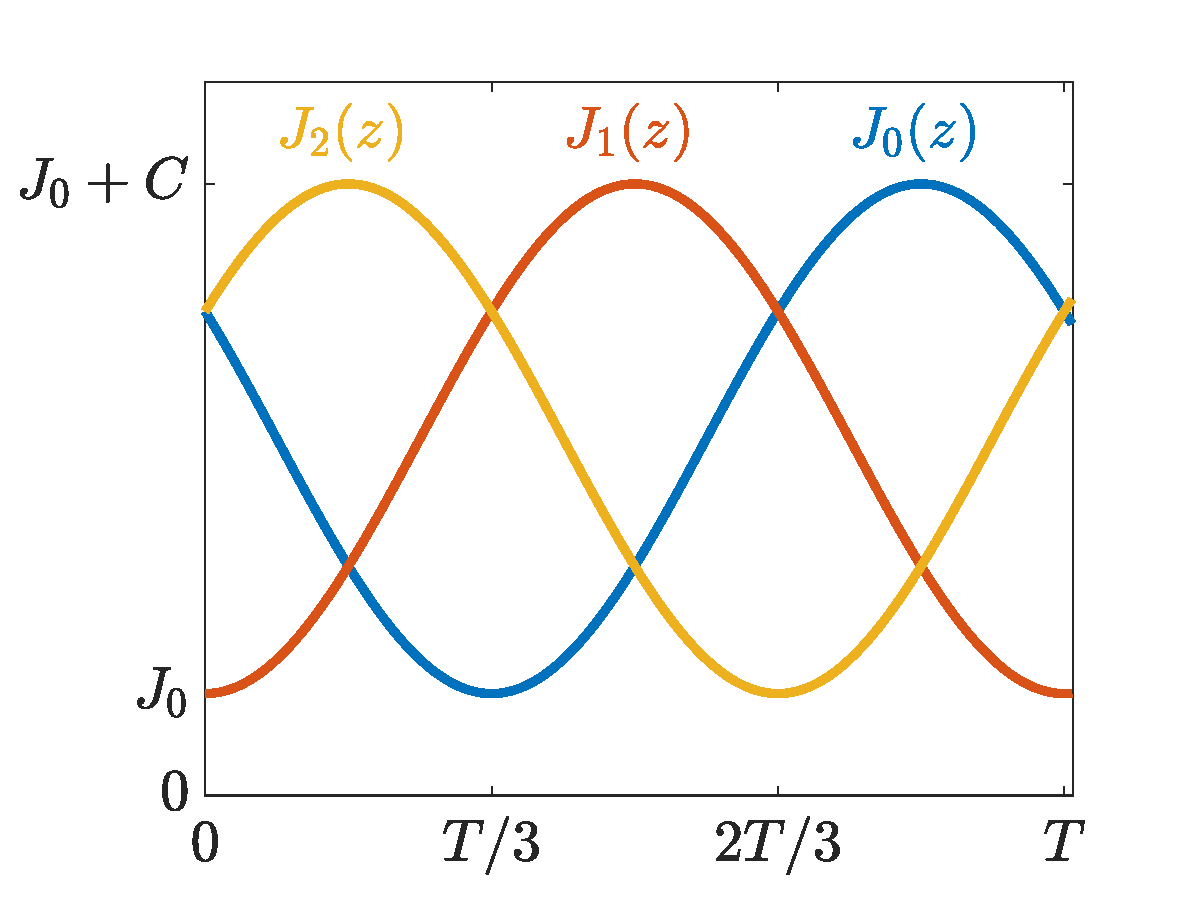
\includegraphics[width=7cm]{J}
    \caption{Coupling function $J_n(z)$ for $n = 0,1,2$.}
    \label{fig:J}
\end{figure}

\section{Evolution from single-site initial conditions}

\begin{figure}[H]
    \centering
    \begin{tabular}{cccc}
    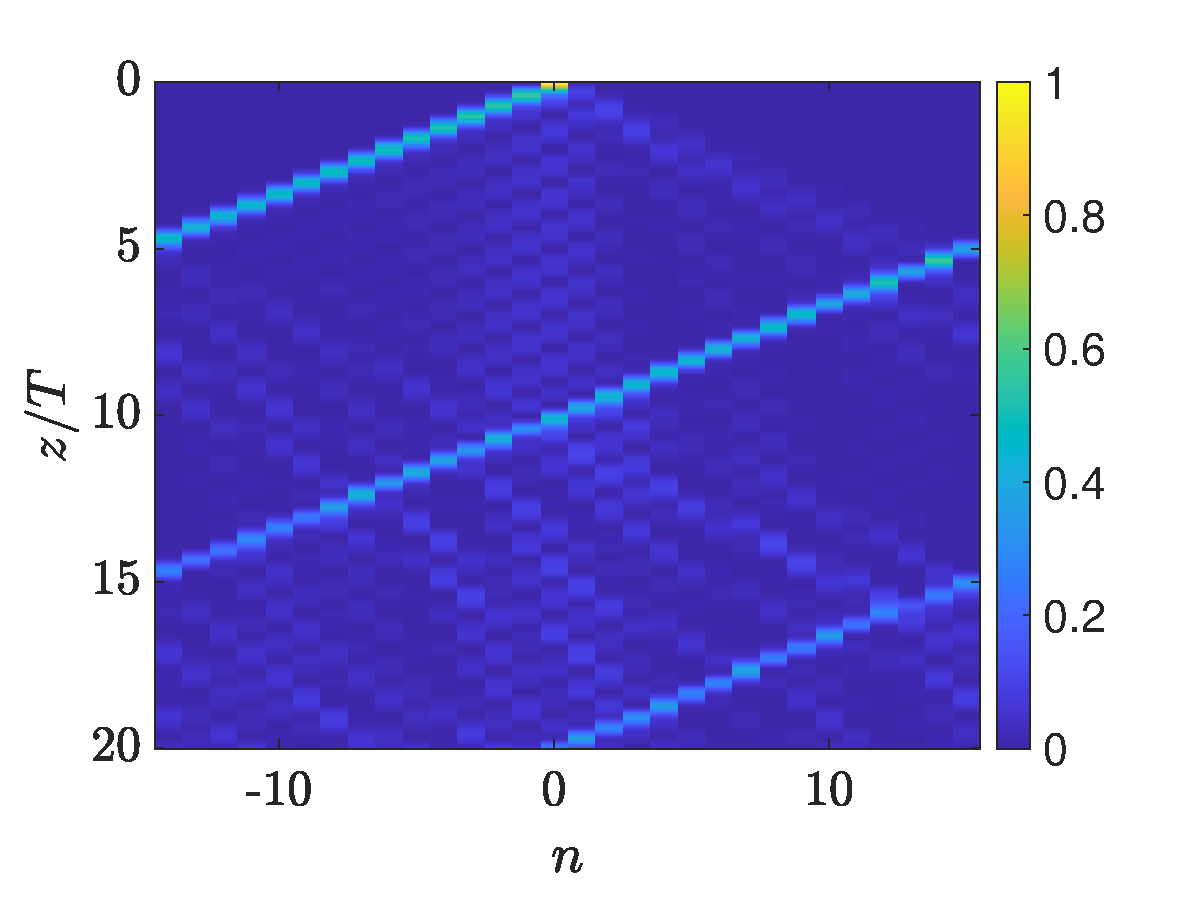
\includegraphics[width=4cm]{left1} &
    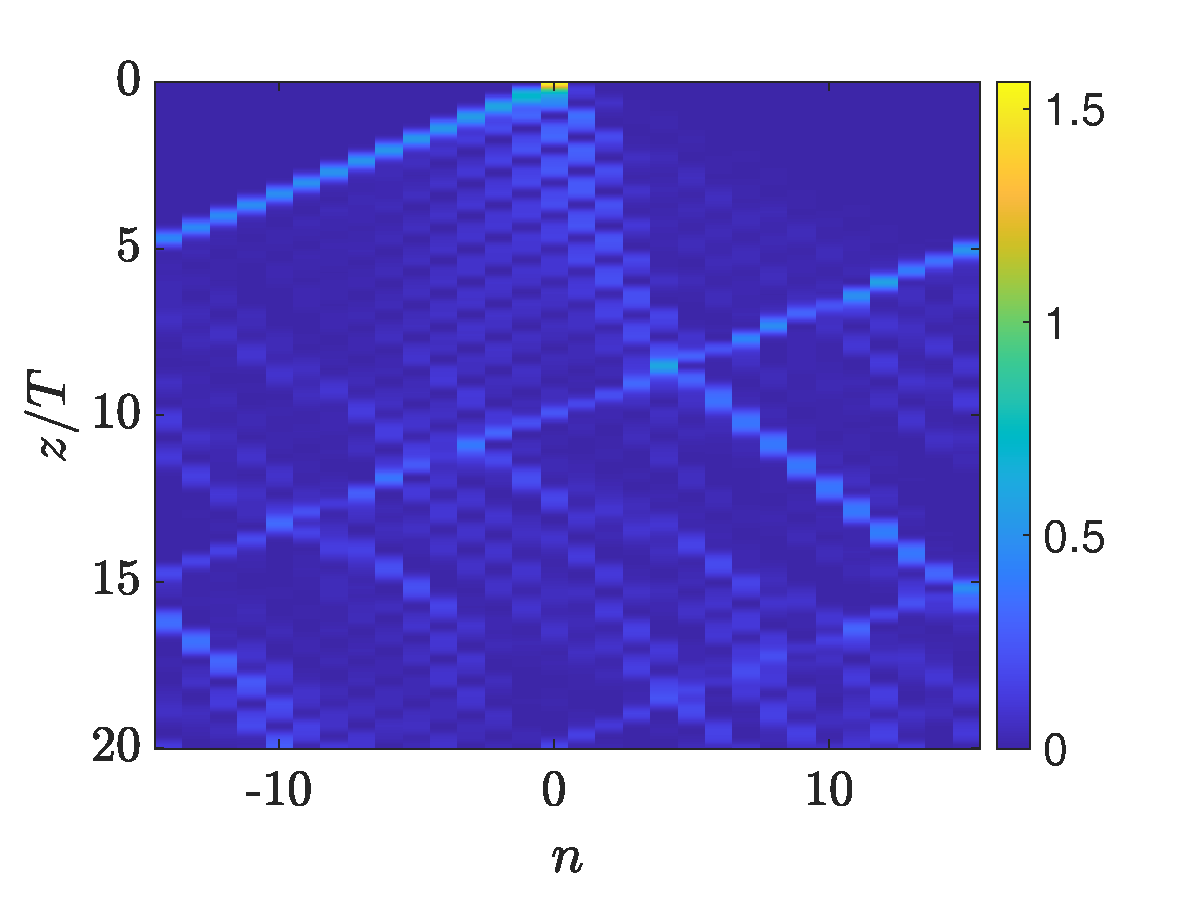
\includegraphics[width=4cm]{left125} &
    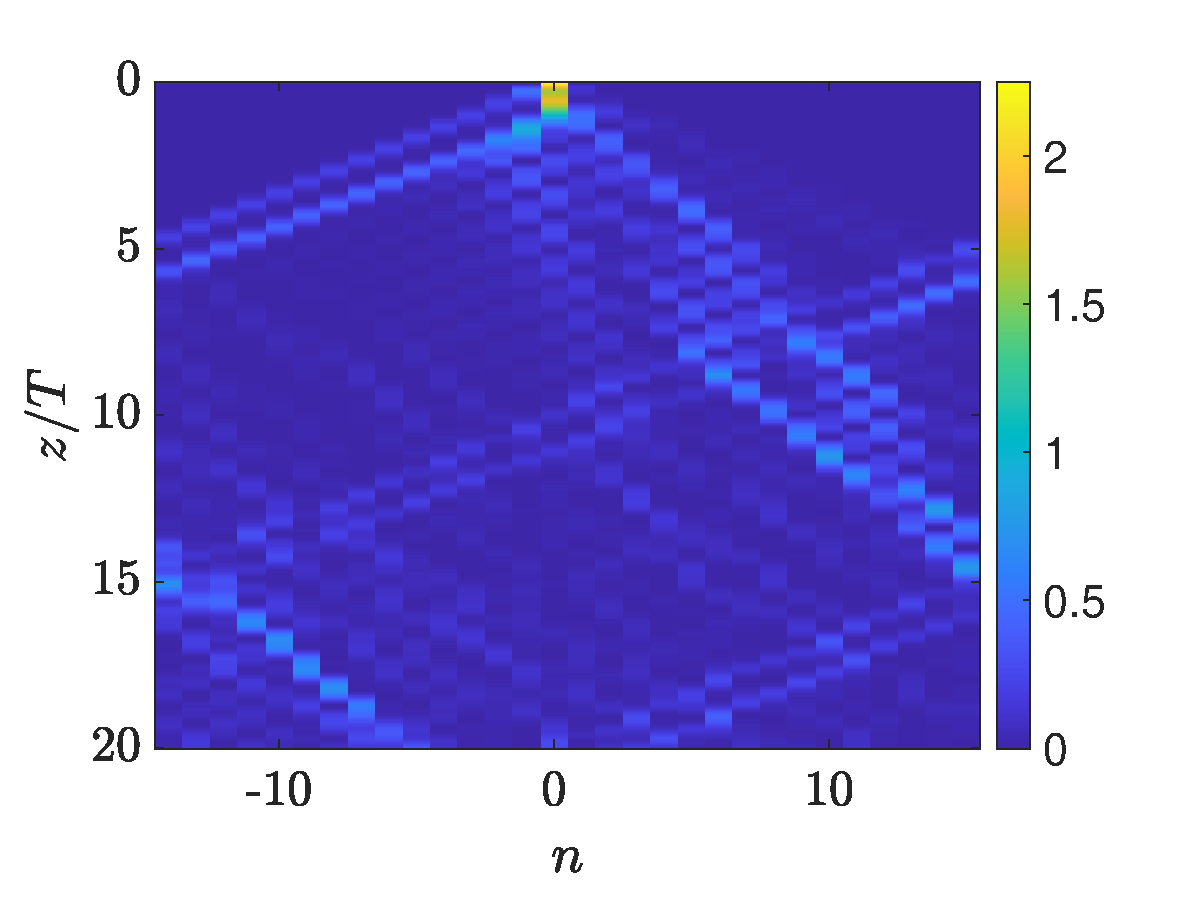
\includegraphics[width=4cm]{left15} &
    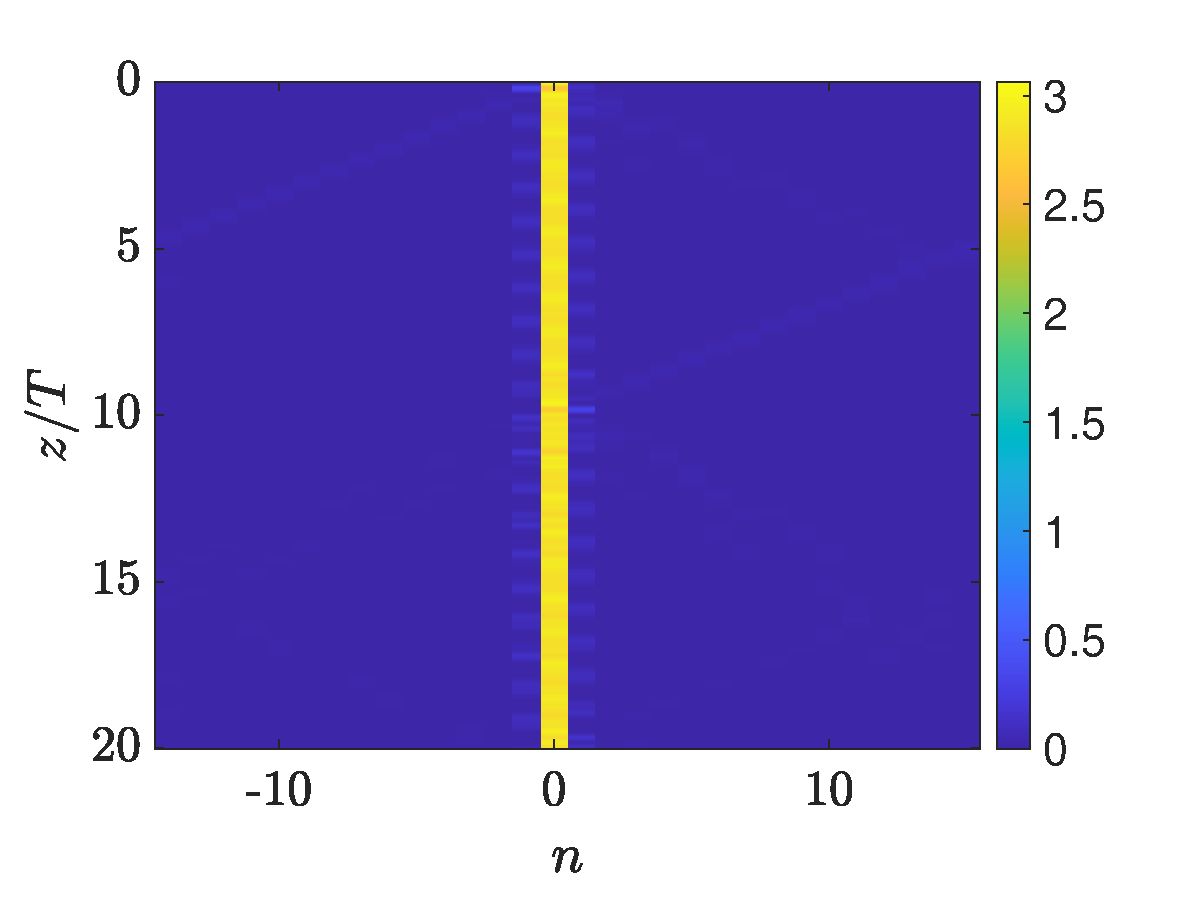
\includegraphics[width=4cm]{left175} \\
    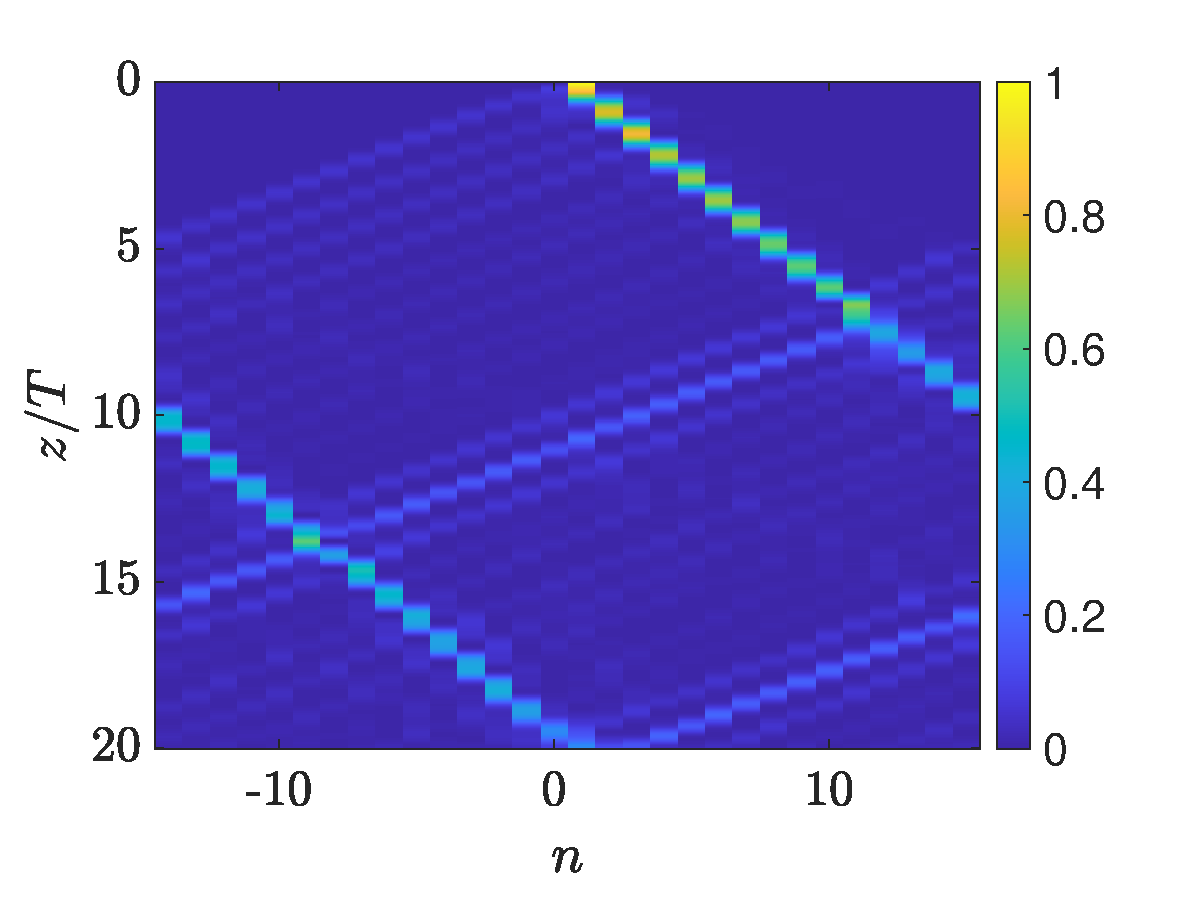
\includegraphics[width=4cm]{right1} &
    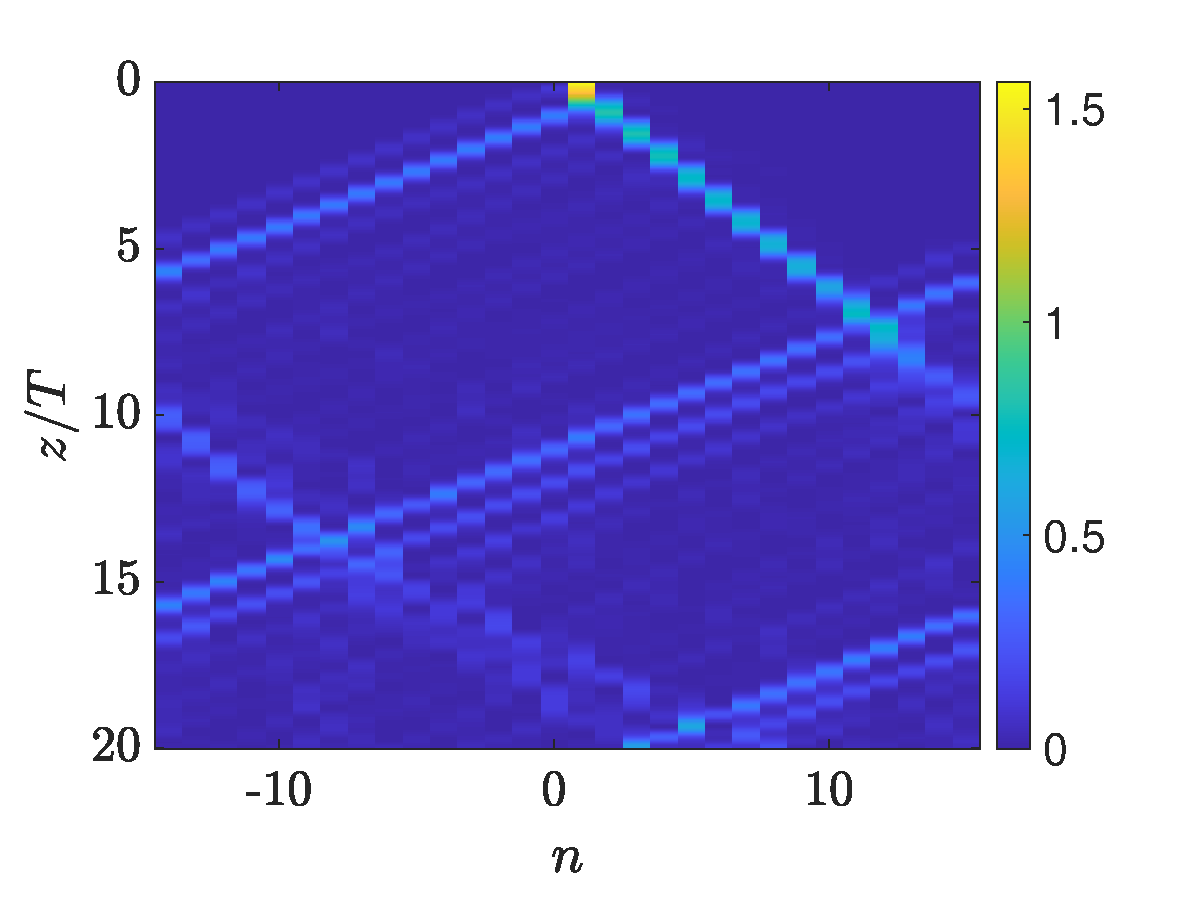
\includegraphics[width=4cm]{right125} &
    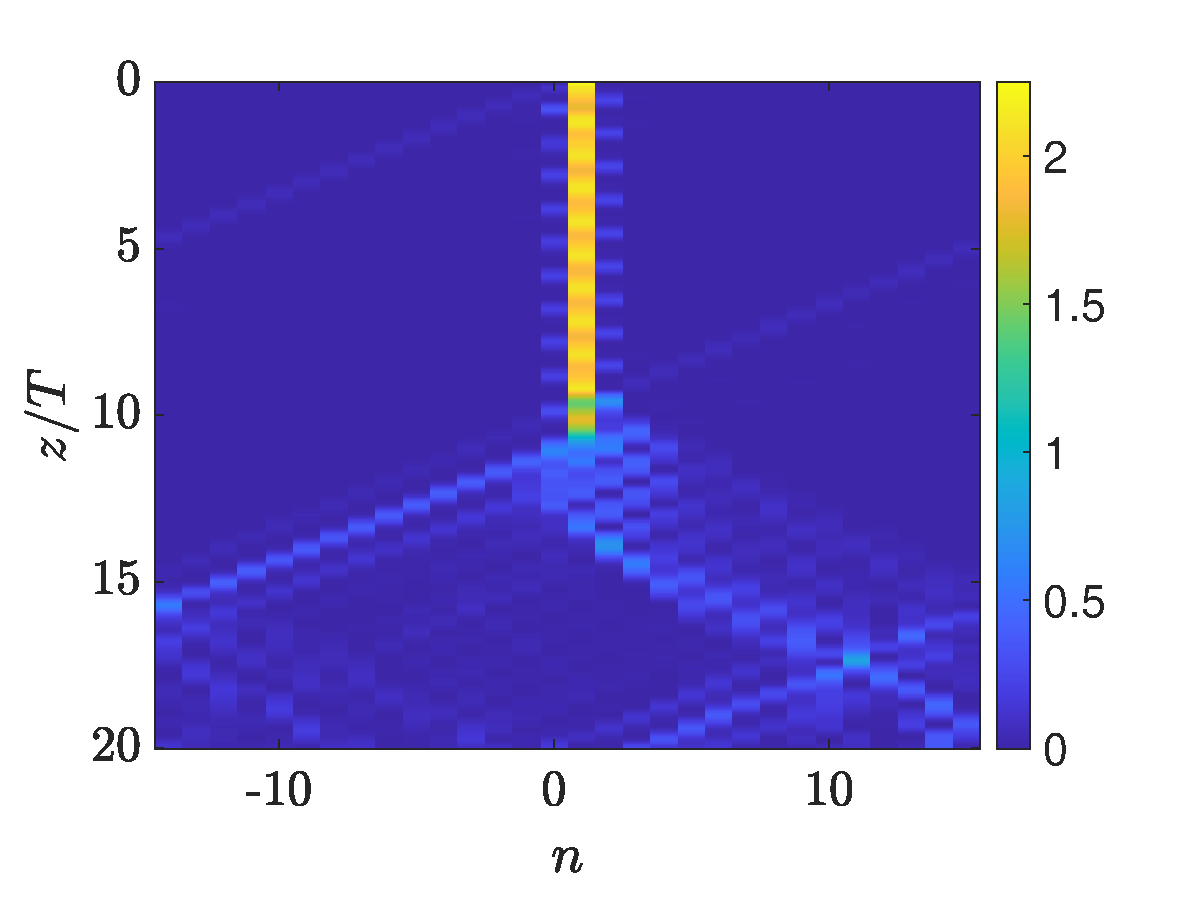
\includegraphics[width=4cm]{right15} &
    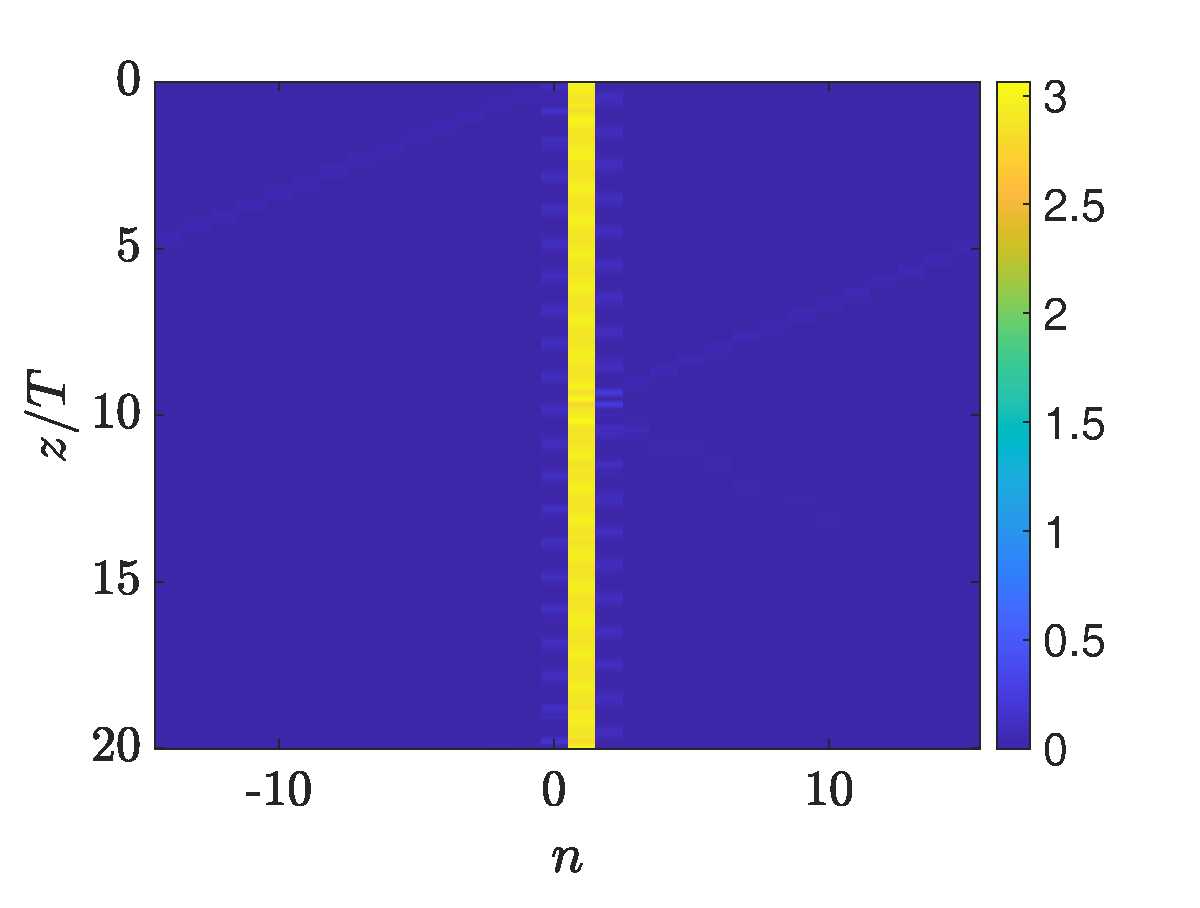
\includegraphics[width=4cm]{right175}
    \end{tabular}
    \caption{Evolution in $z$ of single-site initial condition at lattice site $n=0$ (top) and lattice site $n=1$ (bottom). Initial amplitude (left to right): 1, 1.25, 1.5, 1.75. $J_0 = 0.05$, $C=0.4$, $g=1$, 30 lattice sites. }
    \label{fig:evolmoving}
\end{figure}

\section{Coherent Structures}

Possible coherent structures that can be obtained are left-moving, right-moving, and stationary \cref{fig:coherent}. Left-moving structure moves 3 lattice sites to left in one period, reproduces itself exactly after one period (after one period, it moves one lattice site to the left, with a phase shift of $2\pi/3$). Right-moving structure moves 3 lattice sites to right in two periods, reproduces itself exactly after two period (the one shown reproduces itself exactly after 2/3 period, at which point it has moved one lattice site to the right.) Note the asymmetry of the right-moving solution. Stationary solution reproduces itself exactly after one period.

\begin{figure}[H]
    \centering
    \begin{tabular}{ccc}
    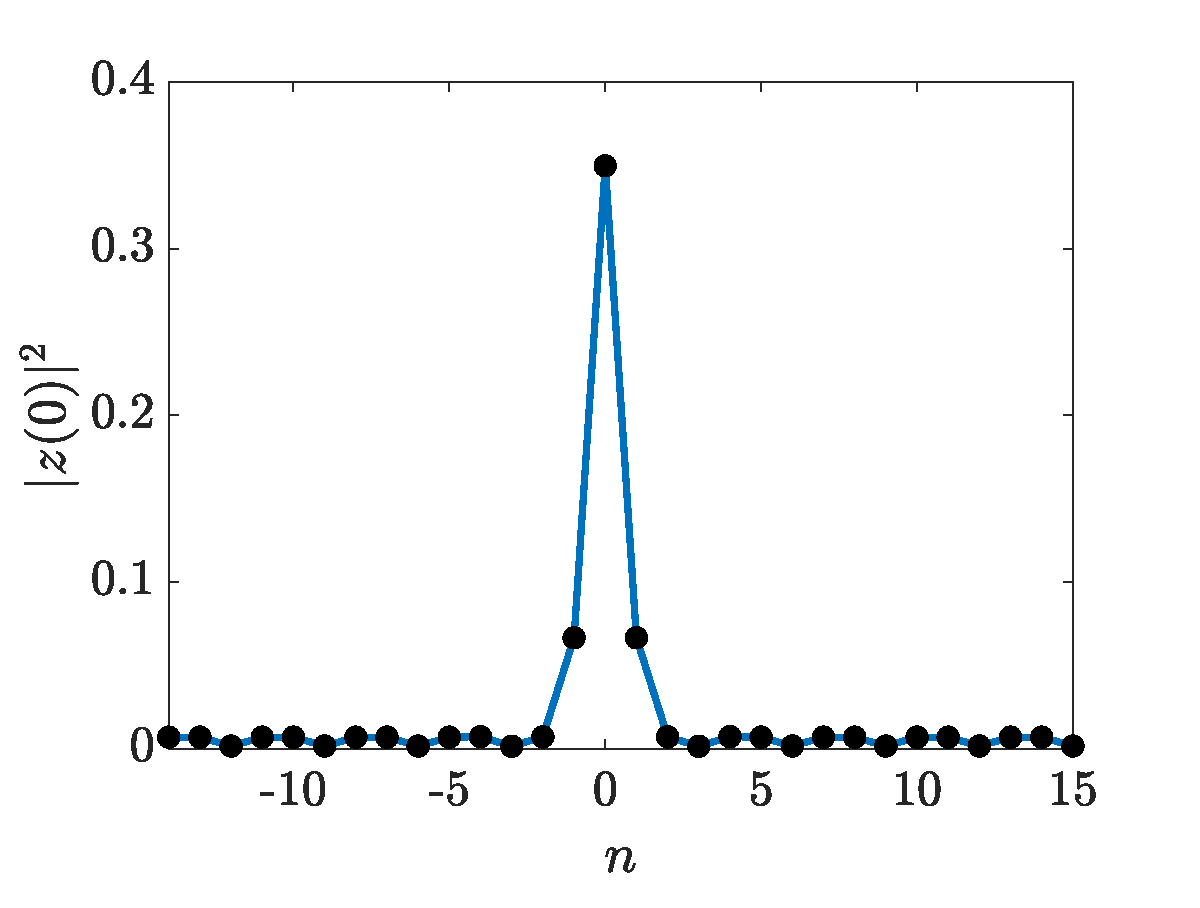
\includegraphics[width=5cm]{leftsol} &
    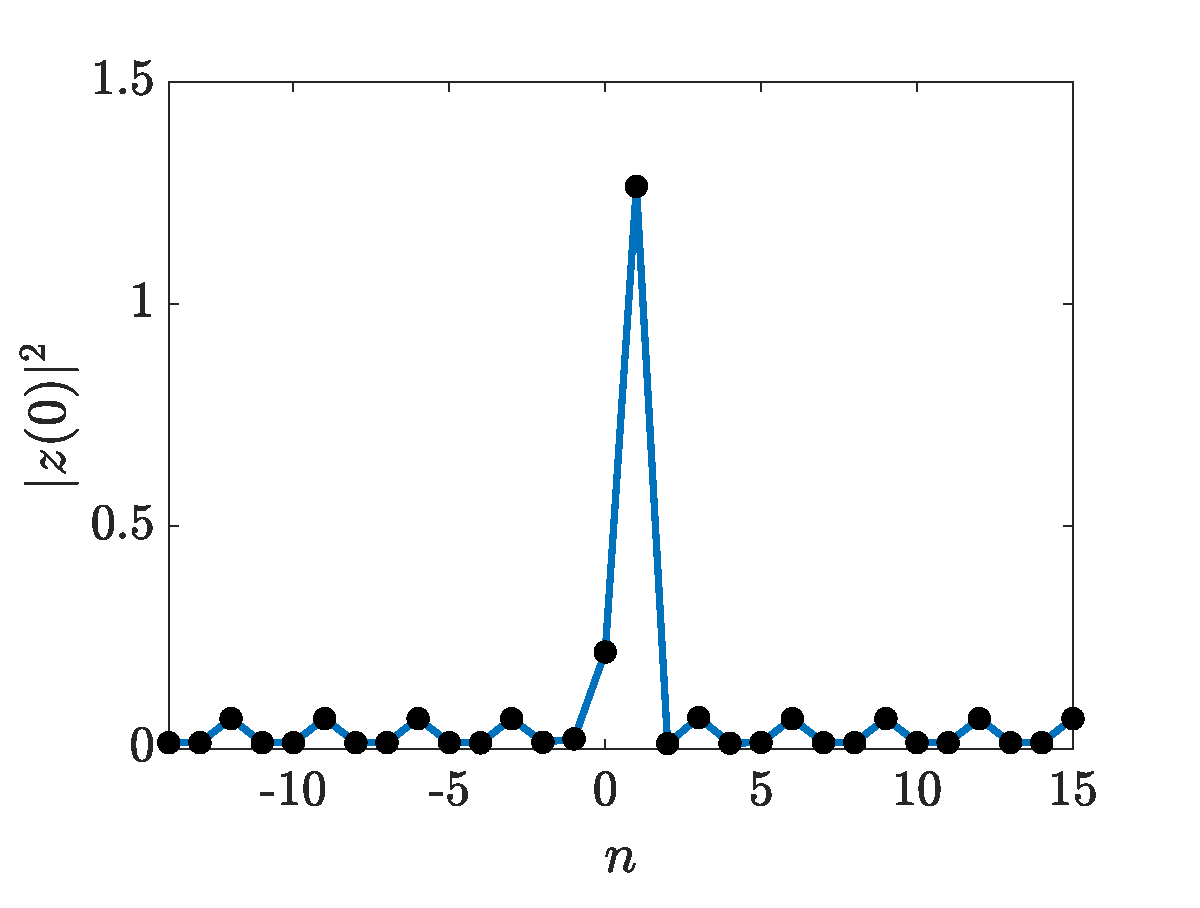
\includegraphics[width=5cm]{rightsol} &
    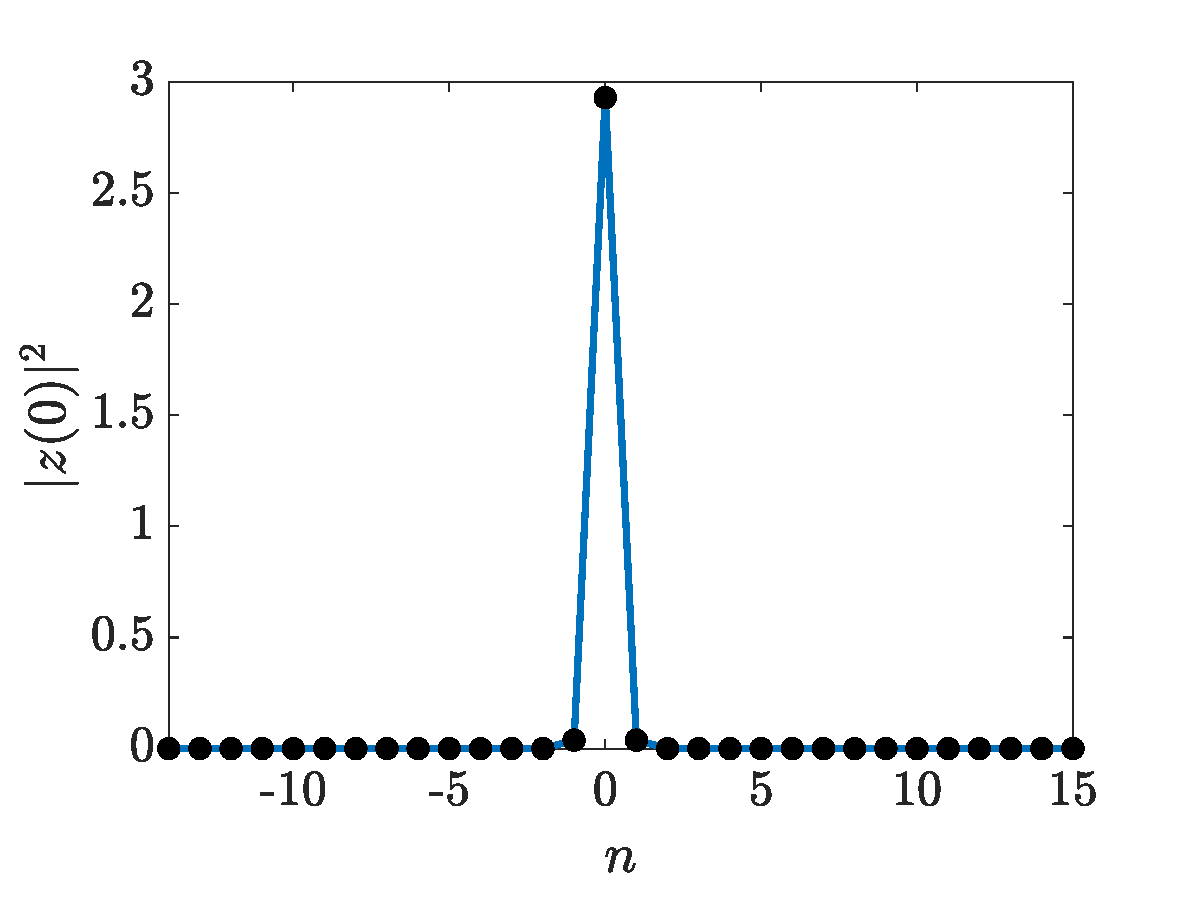
\includegraphics[width=5cm]{statsol} \\
    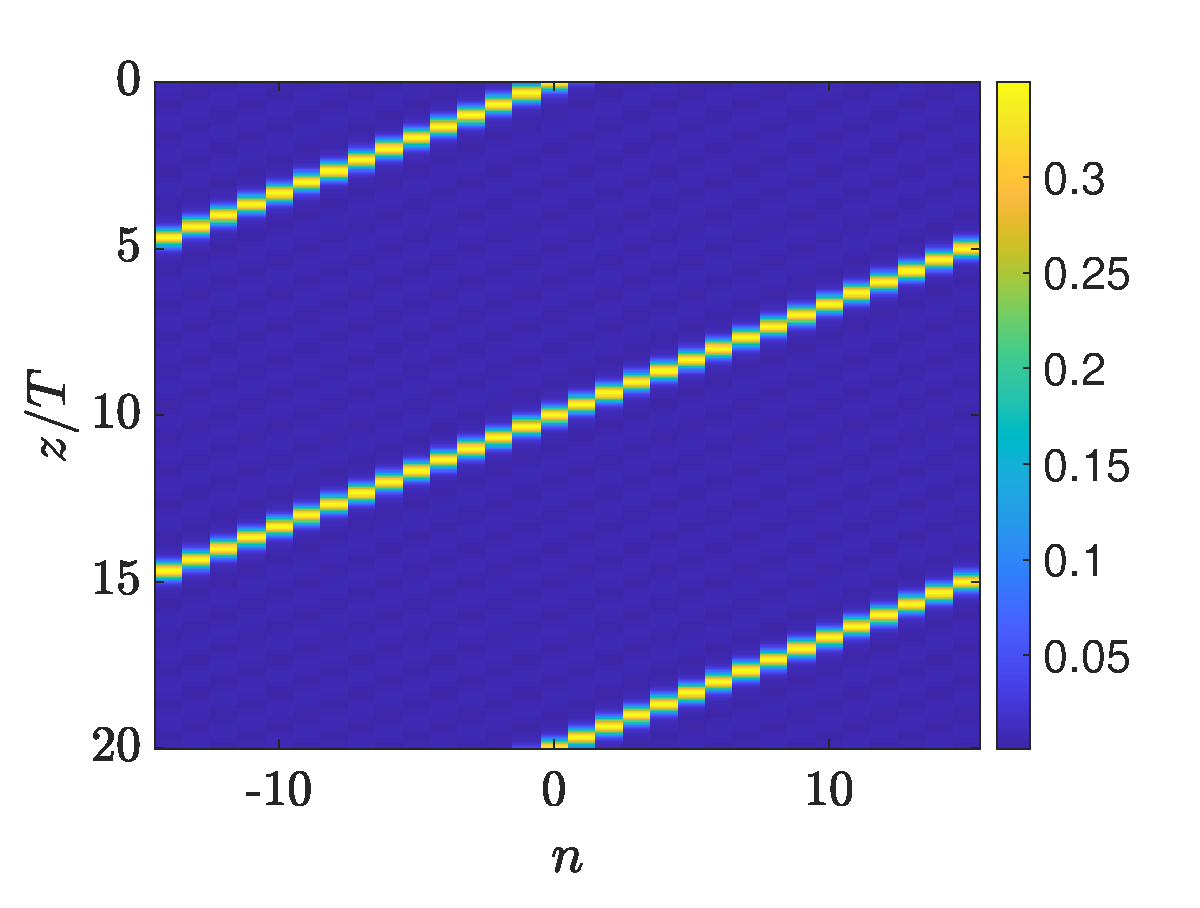
\includegraphics[width=5cm]{leftcolormap} &
    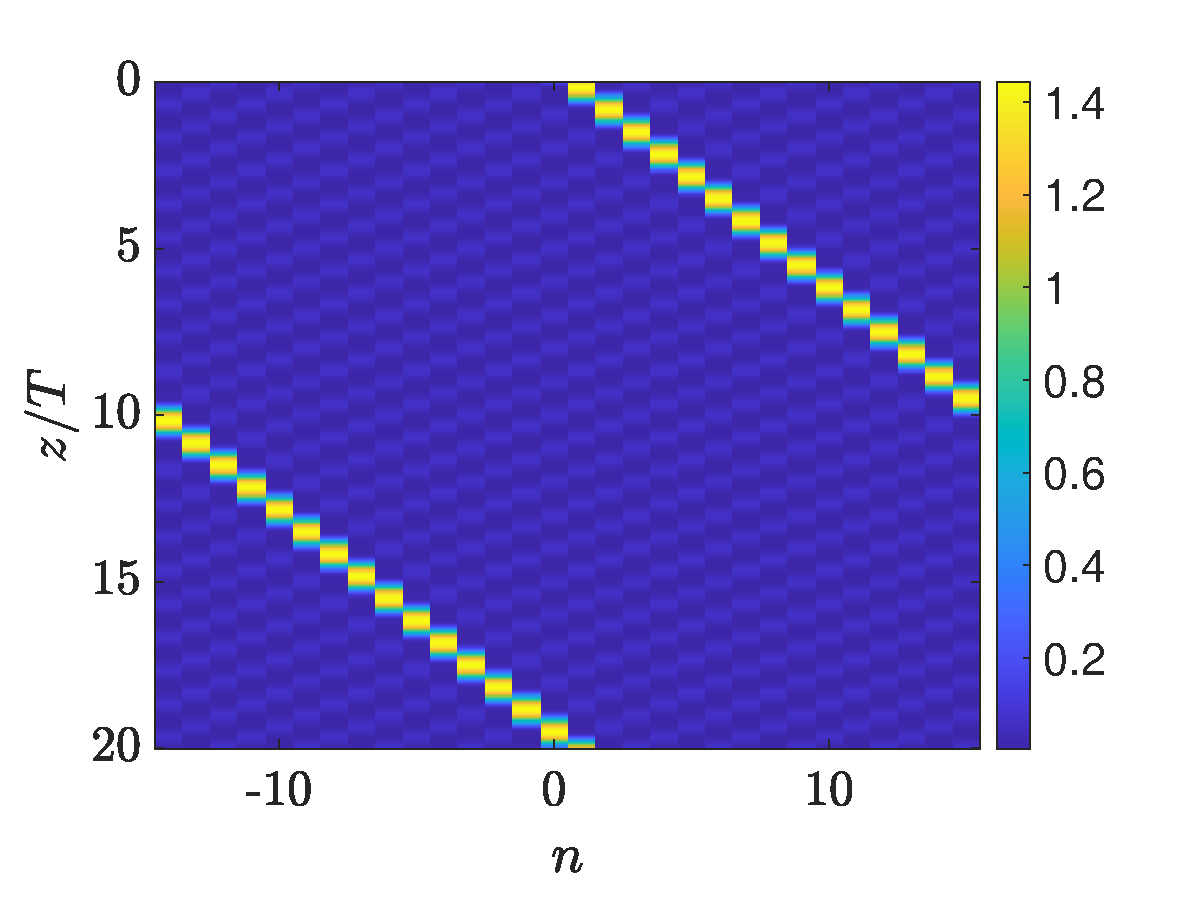
\includegraphics[width=5cm]{rightcolormap} &
    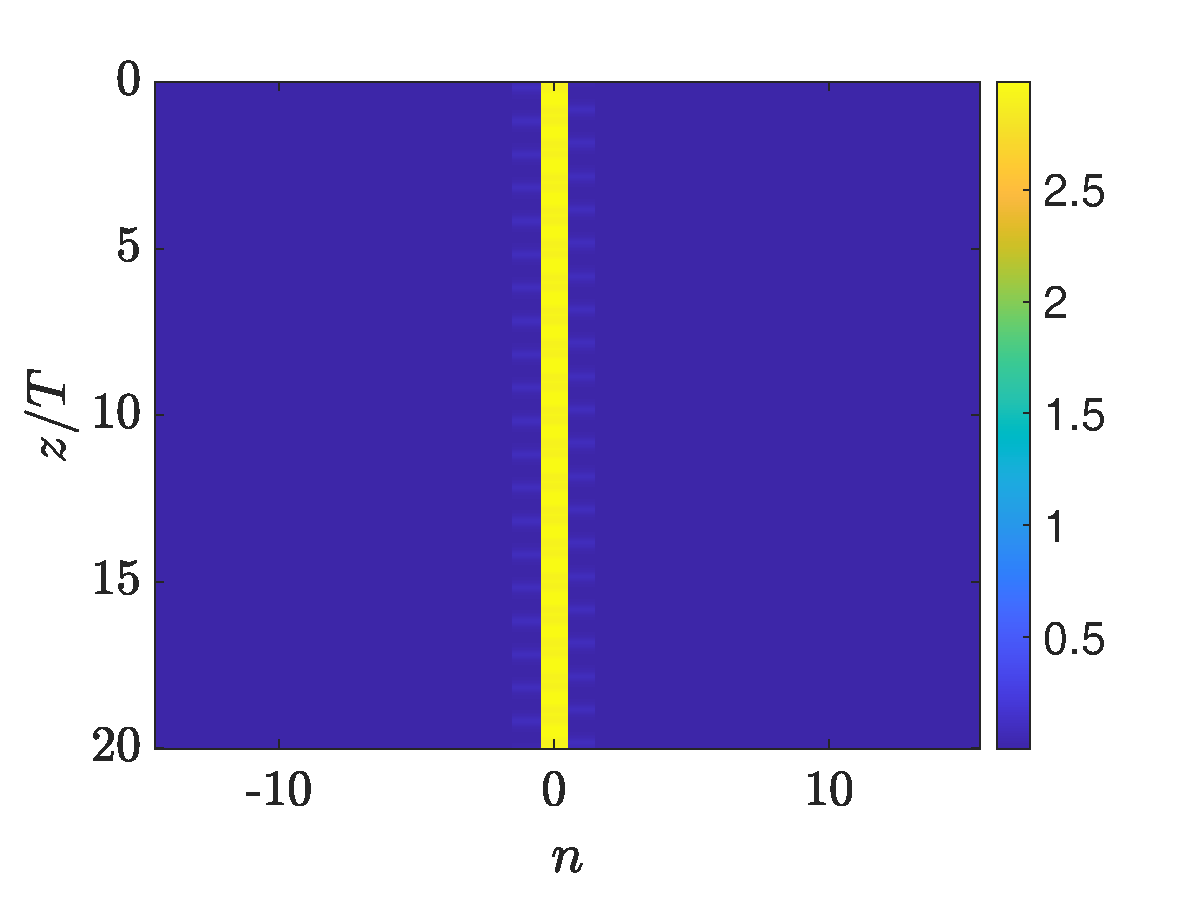
\includegraphics[width=5cm]{statcolormap} 
    \end{tabular}
    \caption{Left-moving, right-moving, and stationary coherent structures. Top is power of solution at $z=0$, bottom is colormap showing evolution of solution in $z$. $J_0 = 0.05$, $C=0.4$, $g=1$, 30 lattice sites.}
    \label{fig:coherent}
\end{figure}






\bibliographystyle{amsplain}
\bibliography{main.bib}

\end{document}